%%%%%%%%%%%%%%%%%%%%%%%%%%%%%%%%%%%%%%%%%%%%%%%%%%%%%%%%%%%%%%%%%%%%%%
%%                       IAEW LaTeX Template                        %%
%%%%%%%%%%%%%%%%%%%%%%%%%%%%%%%%%%%%%%%%%%%%%%%%%%%%%%%%%%%%%%%%%%%%%%
% ANGELEGT am 17.09.2026, Auftrag des Verfassers. Der Fahrplan in Abschnitt 3.3.3 steht
% MIT der Mindestgroesse von 25 MW, hier steht derselbe Tag OHNE sie. Die beiden
% Abbildungen unterscheiden sich in nichts anderem, die Fassung ohne Mindestgroesse
% ist bitgleich mit dem Stand, der bis zum 17.09.2026 in Kapitel 3 stand (s.
% dispatch_festpreis.py im Modellrepository).
\chapter{Fahrplan ohne die Mindestgröße}
\label{anh:dispatch_ohne}

Der Basisfall des Optimierungsmodells kennt keine Mindestgröße der kurativen Reservierung, während der Fahrplan in Abschnitt~\ref{sec:validation_function} die Mindestgröße von 25\,\si{MW} enthält.
% I-46 am 18.09.2026, Kontrolle durch Fable, Entscheidung des Verfassers: der vorgegebene Reservierungspreis ist ein eigener Begriff. Alte Fassung:
%Abbildung~\ref{fig:dispatch_festpreis_ohne} zeigt denselben Liefertag bei demselben Reservierungspreis von 5\,\EurMWh{} ohne diese Mindestgröße.
Abbildung~\ref{fig:dispatch_festpreis_ohne} zeigt denselben Liefertag bei demselben vorgegebenen Reservierungspreis von 5\,\EurMWh{} ohne diese Mindestgröße.
Die beiden Abbildungen unterscheiden sich allein in der Mindestgröße, denn beide Läufe tragen im Übrigen dieselbe Konfiguration.
% BERICHTIGT am 17.09.2026: die kurative Reservierung ist innerhalb der Stunde konstant, die zwoelf Slots der Zeitreihe sind drei Stunden. Beleg: eigene Auswertung von run_20260914_110947. Alte Fassung:
%Ohne die Mindestgröße reserviert die Optimierung auch kleine Ladeleistungen, was an den zwölf Viertelstunden mit weniger als 25\,\si{MW} Ladeleistung zu erkennen ist.
Ohne die Mindestgröße reserviert die Optimierung auch kleine Ladeleistungen, nämlich in drei Stunden weniger als 25\,\si{MW}.

\begin{figure}[H]
    \centering
    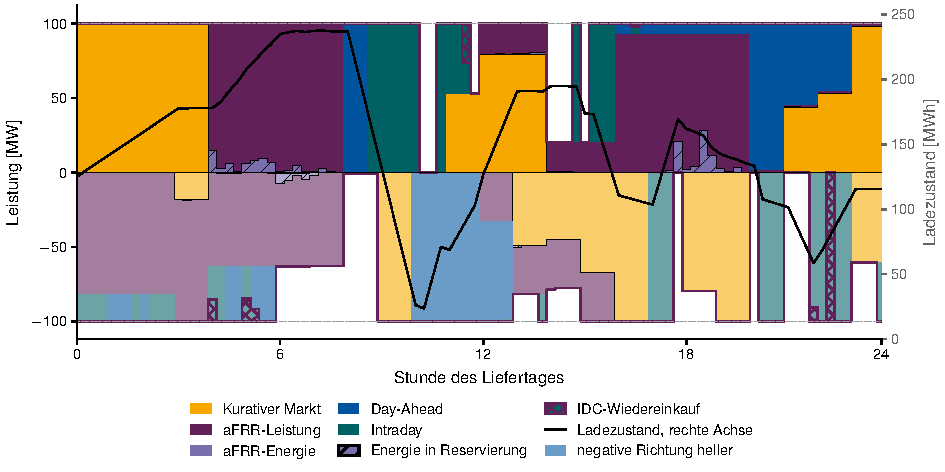
\includegraphics[width=\textwidth]{figures/anhang/dispatch_festpreis_2025-02-11_p5_ohne_mindestgebot.pdf}
% I-46 am 18.09.2026, Kontrolle durch Fable, Entscheidung des Verfassers: der vorgegebene Reservierungspreis ist ein eigener Begriff. Alte Fassung:
%    \caption{Fahrplan und Ladezustand am 11.02.2025 bei einem Reservierungspreis von 5\,\EurMWh{} ohne die Mindestgröße von 25\,\si{MW}, positive Richtung oben, negative Richtung unten.}
    \caption{Fahrplan und Ladezustand am 11.02.2025 bei einem vorgegebenen Reservierungspreis von 5\,\EurMWh{} ohne die Mindestgröße von 25\,\si{MW}, positive Richtung oben, negative Richtung unten.}
    \label{fig:dispatch_festpreis_ohne}
\end{figure}
